\section{Introduction}
Recommender systems help and enhance the natural way people share suggestions with each other. In a usual recommender system, people give recommendations, and the system collects and sends them to the right recipients. Sometimes, the system's main role is in combining the recommendations effectively, while in other cases, it's valuable because it can match the right recommenders with those who are looking for suggestions \cite{resnick1997recommender}. 

When generating recommendations for a specific user, a fundamental yet diverse approach involves selecting items liked by other users who share similarities with the target user. However, the field of recommendation lacks universal "first principles" that can definitively guide the recommendation process. This is evident in the multitude of ways this basic approach can be implemented, with questions arising about how to effectively measure user similarity and evaluate its uncertainty. Challenges also emerge in aggregating varied opinions from different users, handling users with limited available information, and determining the trustworthiness of all data points, including the ability to detect potentially reckless or intentionally misleading opinions. These issues persist even when employing more advanced methods beyond those based solely on user similarity. Fortunately, real datasets are available for experimentation, allowing for the measurement and comparison of individual method performances. Much like physics, it is through experimentation that the effectiveness of a recommendation approach is determined, as there is no one-size-fits-all solution to these complex challenges \cite{lu2012recommender}.

In recent years, the realm of E-learning, also known as online learning, has experienced considerable expansion in response to heightened interest, particularly driven by the lockdowns stemming from the COVID-19 pandemic. This mode of education has emerged as a crucial avenue for acquiring knowledge, catering not only to traditional students in academic institutions but also to lifelong learners seeking improvement in both their social interactions and professional endeavors \cite{salehi2013hybrid}. E-learning platforms offer a diverse array of online courses and learning resources across various disciplines, such as computer science, mathematics, and business. Prominent platforms like Coursera exemplify this trend, providing users with access to courses, degrees, programs, and certificates from esteemed institutions like Stanford and Harvard, as well as leading companies such as Google and IBM. Faced with a multitude of courses and resources, users grapple with the challenge of determining the most beneficial options to advance their careers and remain competitive in the global job market \cite{castro2007applying}. Consequently, the development of recommender systems becomes imperative, offering invaluable assistance to users in navigating the abundance of courses, resources, and learning materials within the E-learning landscape.

\begin{figure}[h]
    \centering
    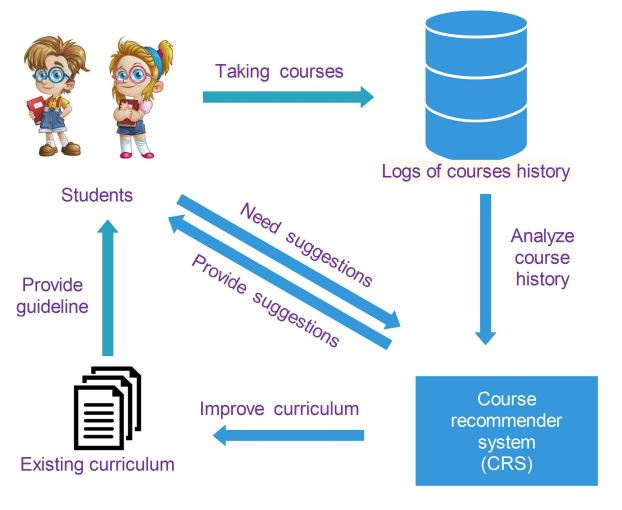
\includegraphics[width=0.8\linewidth]{figures/crs.PNG} 
    \caption{The overall structure of a course recommender system \cite{wang2017sequence}.}
    \label{fig:myimage}
\end{figure}

Compared with classical e-commerce recommendation,
recommender systems have unique characteristics in the context of E-learning:
\begin{enumerate}
    \item Learners' needs and the specifics of learning activities often involve uncertain and ambiguous information. For example, learners might be uncertain about the exact skills or courses they require but have a clear understanding of the type of job they are pursuing. 
    \item The context of learning is important to learners such as the purpose of taking the course and the learning style. The recommendations for full-time learners and fragmentary time learners should be different.
    \item The learning courses, activities, and materials need to be arranged in order to ensure that the prerequisites of some courses are met. A simple example is that, if the course “Software Engineering” needs the prerequisite course “System Analysis and Design”, then it would be unsuitable to recommend the course “Software Engineering” if the learner has not yet taken the course “System Analysis and Design”. 
    \item The need of learners is an adaptive learning route that helps them to gain knowledge continuously. For the life-long learners, what they need is not only one course, but a learning route that contains a package of courses, activities, and materials in an adequate order.
\end{enumerate}
    
Because of these features, people have come up with ways to recommend things for online learning, especially to help those who are learning throughout their lives \cite{zhang2021recommender}.

In this proposal, we present a hybrid method utilizing Autoencoder to address two main challenges: acquiring a nonlinear representation of users and items, and overcoming the cold start issue by incorporating additional information. In comparison to prior models with a similar focus \cite{sedhain2015autorec}, \cite{strub2015collaborative}, \cite{wu2016collaborative}, our framework will consider learners preferences, similarities, and prerequisites within a single matrix. This integration results in enhanced collaborative filtering outcomes.
\begin{figure}[h]
    \centering
    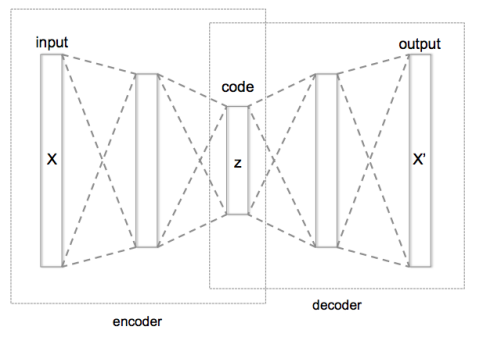
\includegraphics[width=0.6\linewidth]{figures/autoencoder.PNG} 
    \caption{Schematic structure of an Autoencoder with Three fully connected hidden layers. The code (z) is the most internal layer. \cite{darban2022ghrs}.}
    \label{fig:myimage}
\end{figure}

\newpage
\section{Background and Present State}
Over time, the evolution of recommender systems can be categorized into three main stages: shallow models \cite{koren2009matrix} \cite{rendle2010factorization} \cite{rendle2012bpr}, neural models \cite{cheng2016wide} \cite{guo2017deepfm} \cite{he2017neural}, and GNN-based models \cite{he2020lightgcn} \cite{wang2019neural} \cite{ying2018graph}. Initially, recommendation models centered on collaborative filtering, gauging interaction similarities directly . To refine this, model-based CF methods like matrix factorization \cite{koren2009matrix} and factorization machines \cite{rendle2010factorization} were introduced, treating recommendation as a representation learning problem. However, these approaches faced challenges related to complex user behaviors and data input.

In response to these challenges, neural network-based models \cite{cheng2016wide} \cite{guo2017deepfm} \cite{he2017neural} emerged, introducing innovations such as neural collaborative filtering (NCF), which extended traditional models by incorporating multi-layer perceptrons (MLP) to enhance capacity. Deep factorization machine (DeepFM) \cite{guo2017deepfm} took a similar approach, combining shallow models like factorization machines \cite{rendle2010factorization} with MLP. Despite these advancements, these methods remained limited, primarily because their prediction and training paradigms overlooked high-order structural information in the observed data. For instance, NCF's optimization goal focused on predicting user-item interactions, considering observed positive and unobserved negative interactions. This meant that during parameter updating for a specific user, only the items they interacted with were considered \cite{gao2023survey}.

Recently, the advent of graph neural networks (GNNs) has offered a compelling opportunity to address these limitations in recommender systems. GNNs leverage embedding propagation, iteratively aggregating neighborhood information. By stacking these propagation layers, each node gains access to high-order neighbors' information, surpassing the constraints of traditional methods that only consider first-order neighbors. With their proficiency in handling structural data and exploring intricate information, GNN-based methods have emerged as the new cutting-edge approaches in the field of recommender systems \cite{gao2023survey}.

Deep learning, a subset of machine learning research, involves the acquisition of multiple levels of representations and abstractions from data, proving effective in addressing both supervised and unsupervised learning tasks. Existing recommendation models within the deep learning framework can be categorized into two classes based on the employed deep learning approaches\cite{zhang2019deep}:
\begin{enumerate}
    \item \textbf{Recommendation with Neural Building Blocks:} In this class, the applicability of the recommendation model is determined by the deep learning technique employed. For instance, Multi-Layer Perceptrons (MLP) can model non-linear interactions between users and items; Convolutional Neural Networks (CNNs) extract local and global representations from diverse data sources such as text and images; and Recurrent Neural Networks (RNNs) enable the modeling of temporal dynamics and sequential evolution of content information in recommender systems.
    \item \textbf{Recommendation with Deep Hybrid Models:} Some recommendation models based on deep learning utilize multiple deep learning techniques. The flexibility of deep neural networks allows the combination of various neural building blocks to complement each other, forming a more robust hybrid model. While numerous combinations of these deep learning techniques are possible, not all have been thoroughly explored.
\end{enumerate}

In the field of unsupervised machine learning, Autoencoders play a pivotal role, especially in feature representation and dimensionality reduction, as detailed by Zhang et al.\cite{zhang2019deep}. An Autoencoder's primary objective is to reconstruct its input data (X) in the output layer (X'), utilizing a bottleneck layer (Z) that serves as a crucial feature representation of the input.

Several variants of Autoencoders are recognized, including denoising Autoencoder, marginalized denoising Autoencoder, sparse Autoencoder, contractive Autoencoder, and variational Autoencoder, as outlined by Goodfellow et al.\cite{graves2013speech}. These variants offer diverse approaches to handling data within the Autoencoder framework.

In the specific context of recommender systems, Zhang et al.\cite{zhang2019deep} discuss two principal applications of Autoencoders: firstly, using the bottleneck layer to learn lower-dimensional feature representations, and secondly, employing the reconstruction layer to directly complete the interaction matrix. This adaptability of Autoencoders, encompassing a range of variants like denoising, variational, contractive, and marginalized Autoencoders, makes them highly applicable to tasks in recommender systems. Zhang et al.\cite{zhang2019deep} emphasize employing the first approach, i.e., extracting new low-dimension features using the bottleneck layer of the Autoencoder, and illustrate different recommendation model structures based on this framework.



\section{Research Questions}
The following questions may arise while executing our proposed works:
\begin{itemize}
    \item How does the graph-based hybrid recommendation system compare to traditional shallow models and neural models?
    \item How well does the graph-based hybrid recommendation system perform in practical scenarios?
    \item How do the graph-based models effectively handle sparse data and cold-start problems in recommendation systems?
    \item How do graph-based hybrid systems scale with increasing data size and user/item dimensions?
\end{itemize}
    

\section{Specific Objectives}
The following objectives will be achieved by the execution of the proposed work:
\begin{itemize}
    \item To implement a personalized recommendation system to enhance user engagement and satisfaction on the e-learning platform. 
    \item To develop algorithms that analyze user behavior and preferences to recommend relevant courses, modules, or learning materials to individual users.
    \item To provide personalized learning paths by suggesting a sequence of courses based on a user's skill level, interests, and learning goals.
\end{itemize}

\section{Possible Outcomes}
The are some possible outcomes to be mentioned:
\begin{itemize}
    \item The proposed GHRS could enhance the accuracy of recommendations by combining user preferences derived from a graph-based model, demographic data and Autoencoder-generated features.
    \item Course completion rates could be higher by measuring  the impact of the recommendation system on course completion rates and assess how personalized recommendations influence user behavior.
    \item The proposed recommendation system could mitigate the cold-start problem, a challenge for many recommender systems, by efficiently leveraging users' side information like demographics and locations.
\end{itemize}

\section{Impact Identification}
\subsection{Improved Recommendation Accuracy}
The proposed GHRS could enhance the accuracy of recommendations. By combining user preferences derived from a graph-based model, demographic data, and Autoencoder-generated features, it outperformed various existing algorithms.
\subsection{Addressing the Cold-Start Problem}
GHRS showed promising results in tackling the "cold-start problem," where traditional systems struggle to provide recommendations for new users or items lacking sufficient data. 
\subsection{Enhanced Utilization of User Information}
Utilizing users' demographic and location data alongside their preferences and ratings could potentially lead to more personalized and context-aware recommendations. This means recommendations could align more closely with users' diverse backgrounds and preferences.

\section{Outline of Methodology}
In the realm of personalized recommendation systems for e-learning platforms, leveraging machine learning techniques is essential to enhance the user experience. One powerful methodology for achieving this is the application of K-means clustering. This method allows the platform to group users and items based on their characteristics, facilitating the delivery of tailored recommendations to users with similar preferences.

\begin{figure}[h]
    \centering
    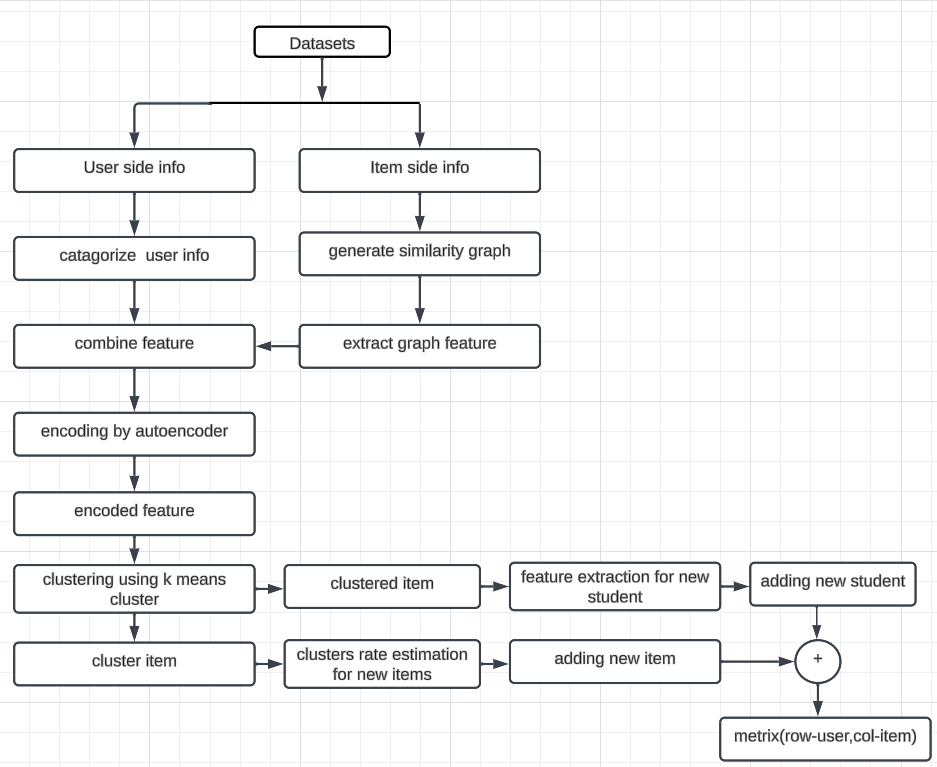
\includegraphics[width=1\linewidth]{figures/proposal methodology.png}
    \caption{Proposed methodology for graph based hybrid recommendation system}
    \label{fig:enter-label}
\end{figure}
\subsection{Dataset}
The dataset is divided into two parts user side information and item side information. then user-side information set is categorized and the side information set is generated in a similarity graph.
\subsection{Combine feature}
Item side information set after generating in similarity graph is extracted in a graph feature. Then categorized user information and extracted graph feature is combined together.
\subsection{Encoding}
After combining item side and user side information datasets the combined dataset is encoded by an autoencoder. And added an encoded feature.
\subsection{Clustering}
For clustering the encoded datasets we used k means cluster. K-means clustering is a popular unsupervised machine learning algorithm used for partitioning a dataset into a set of distinct, non-overlapping subgroups or clusters. The goal of the K-means algorithm is to group data points into K clusters, where each data point belongs to the cluster with the nearest mean.
\subsection{Adding new item and student}
After clustering if we have new student and item we added them in different sets of clusterd item information and clustered student information
\subsection{Adding two clustered information set}
After adding new student and new item there will be new item information dataset and new student information dataset. For running the model we added these dataset together and made a metrics where row is for user or student and column is for item.


\section{Required Resources}
The necessary tools to implement this project can be divided into two Categories- Hardware and Software as illustrated below:  
\begin{itemize}
    \item Personal Computer with Operating System 
    \item Python IDE
    \item Google Colaboratory or Jupyter Notebook
    \item Smart Mobile or Camera
\end{itemize}

\section{Cost Estimation}
Cost estimation is shown here. This estimation may change according to need.\\
Cost of Materials:
\begin{itemize}[label=\textbullet]
  \item Paper \hspace{4.5cm} Tk 500
  \item Drafting \hspace{4cm} Tk 1000
  \item Printing \hspace{4cm} Tk 500
  \item Binding \hspace{4cm} Tk 400
  \item Internet \hspace{4cm} Tk 2000
\end{itemize}

\rule{\linewidth}{1pt}
Total \hspace{5.4cm} Tk 4400
\section{Time Management}
\begin{figure}[h]
    \centering
    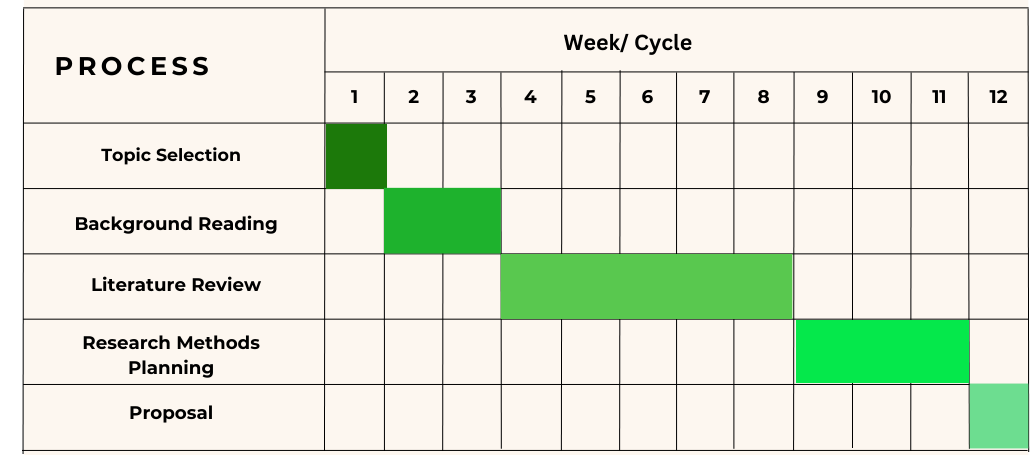
\includegraphics[width=1\linewidth]{figures/Mon.png} 
    \caption{Gantt Chart for Proposal Timeline}
    \label{fig:myimage}
\end{figure}


\section{SWOT Analysis}
\subsection{Strengths}
\begin{enumerate}
    \item Utilizing deep learning and autoencoders may put the project at the forefront of modern AI techniques, offering advanced analytical capabilities.
    \item The system can provide highly personalized recommendations, enhancing user experience in e-learning environments.
    \item Graph-based systems excel in managing complex, interconnected data, which is typical in e-learning scenarios.
    \item Deep learning models, including autoencoders, can handle large datasets, making the system scalable and adaptable to growing e-learning environments.
\end{enumerate}
\subsection{Weaknesses}
\begin{enumerate}
    \item The integration of deep learning with graph-based systems can be technically challenging and may require specialized knowledge.
    \item Effective training of deep learning models often requires large amounts of data, which might be a limitation in certain e-learning contexts.
    \item Such systems can be computationally expensive, requiring significant processing power and potentially leading to higher operational costs.
    \item Deep learning models, if not properly regulated, can overfit to the training data, leading to poor generalization on new, unseen data.
\end{enumerate}
\subsection{Opportunities}
\begin{enumerate}
    \item This project can contribute valuable insights and advancements in the field of AI in education.
    \item With the increasing adoption of e-learning platforms, especially post-pandemic, there is a growing market for advanced recommender systems.
\end{enumerate}
\subsection{Threats}
\begin{enumerate}
    \item Handling sensitive educational data requires adherence to privacy laws and regulations, which can be complex.
    \item The AI-driven recommendation system market is highly competitive, with many established players.
    \item The fast-paced evolution in AI and machine learning might require continual updates and adaptations of the system.
\end{enumerate}
